\documentclass[11pt,a4paper,twocolumn]{article}
\usepackage[french]{babel}
\usepackage[utf8]{inputenc}
\usepackage[T1]{fontenc}
\usepackage{amsmath}
\usepackage{amsfonts}
\usepackage{amssymb}
\usepackage{float}
\usepackage{graphicx}

\usepackage{geometry}
\geometry{tmargin=25mm,bmargin=25mm,lmargin=25mm,rmargin=25mm}

\begin{document}

\title{PACT - groupe 3.2\\Module de détection de déchets\\Rapport PAN 2}
\author{Victor Masiak\\ Nicolas Jow}
\date{\today}

\maketitle

\section{Objectif du module}

\paragraph*{}

L'objectif de notre groupe PACT est de mettre au point un robot éducatif qui, au travers d'activités pédagogiques, sensibilisera les enfants au tris sélectif. Pour ce faire, il devra être capable de repérer et classifier les déchets présents dans son environnement, à l’aide d’une caméra numérique.

\paragraph*{}

L’objectif de ce module est alors la mise au point d’un système d’intelligence artificielle permettant de transformer les données brutes de la caméra (ie des images) en données exploitables par le robot (ie les positions relatives des déchets par rapport au robot, ainsi que leur type).


\section{Ce que l'on a fait}

\paragraph*{}

Nous avons tout d’abord commencé par nous documenter sur les réseaux de neurones en général, sur internet. Nous avons compris le fonctionnement d’un neurone, comment plusieurs neurones peuvent être reliés pour former un réseau neuronal multicouche, les différents algorithmes d'entraînement, etc.
Nous avons rapidement compris que nous allions avoir besoin de récupérer un réseau pré-entraîné, pour ensuite le ré-entraîner sur des images appropriées. Nous nous sommes donc mis à la recherche d’un tel réseau.

\paragraph*{}

Nous sommes tout d’abord tombé sur un projet assez complet\footnote{https://pythonawesome.com/a-growing-image-dataset-of-waste-in-the-wild/}, contenant une implémentation du réseau Mask-RCNN ainsi qu’une base de données de divers détritus dans la nature. Nous avons essayé de comprendre son fonctionnement et de le tester, mais nous avons finalement abandonné cette piste pour deux raisons :

Nous avons trouvé très peu de documentation sur internet. Hors, nous avons rencontré de multiples problèmes d’installation des différentes dépendances, que nous n’avons pas réussi à résoudre complètement.

Le projet est très complet, et donc déjà fini et fonctionnel. Par conséquent, nous n’aurions eu que très peu de travail, celui-ci se limitant à télécharger le projet et ses dépendances.

\paragraph*{}

Nous avons alors trouvé le réseau Inception, pré-entraîné sur la banque d’images xxx. Après nous être documenté sur internet, il semble que ce réseau soit très performant, et adapté à notre situation.
Nous avons donc cherché une base d’images de déchets pour pouvoir ré-entraîner le réseau. Nous avons trouvé une base d’images sur un challenge kaggle\footnote{https://www.kaggle.com/asdasdasasdas/garbage-classification/data} disposant de six classes : carton, verre, métal, papier, plastique et non recyclable. Cette base de données nous a semblé correspondre parfaitement à nos besoin, mais nous avions cependant des toutes sur sa taille (environ 500 images par catégorie, ce qui nous semblait peu).
Nous avons donc suivi un tutoriel du site de tensoflow\footnote{https://www.tensorflow.org/hub/tutorials/image\textunderscore retraining} pour ré-entraîner la dernière couche du réseau avec notre base de données. Les résultats sont présentés dans la figure \ref{entropy} :

\begin{figure}[H]
	\center
	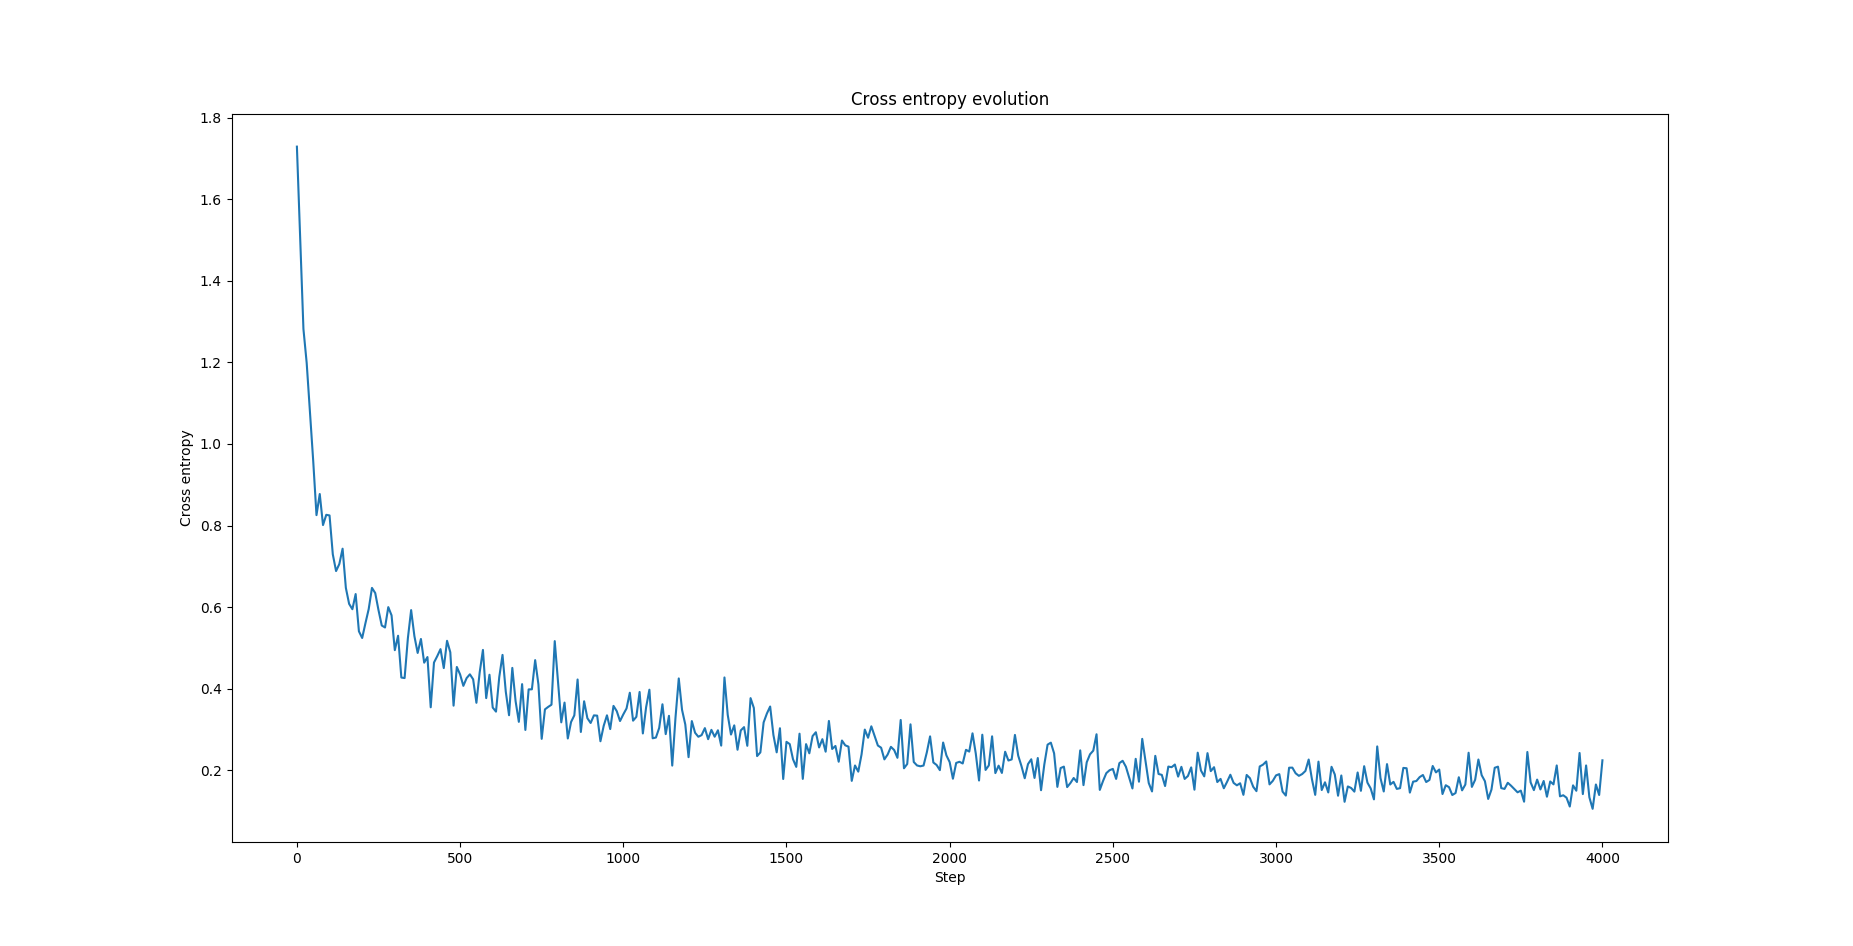
\includegraphics[width=7cm]{entropy.png}
	\caption{Ré-entraînement de la dernière couche du réseau Inception sur notre BDD}
	\label{entropy}
\end{figure}

\paragraph*{}

Après entraînement, le taux d’erreurs du réseau est d’environ 10\%. Ce premier résultat est satisfaisant, surtout si on prend en compte la complexité de certains déchets, qui peuvent être interprétés de différentes manières (la BDD contient par exemple des feuilles de magazines plastifiés, que l’on pourrait classer comme du papier mais aussi comme du plastique). Nous avons de plus repéré quelques images mal labellisées. Nous espérons néanmoins réduire ce taux d’erreurs dans le futur.

\paragraph*{}

Nous nous sommes ensuite intéressés au cas ou l’image contient plusieurs déchets, qui ne sont pas centrés sur l’image. Nous avons pour cela choisi de balayer l’image, et d’appliquer le réseau sur des portions extraites de l’image, pour sélectionner celles qui produisent une réponse forte de l’une des classes. Néanmoins, le réseau passe plusieurs fois sur chaque déchets (à différentes échelles, de manière plus ou moins centrée, etc.), et il faut donc ensuite trier les coordonnées retournées. Nous avons pour cela décidé d’effectuer un barycentre pour chacune des classes.
Cette méthode nous a donné des résultats plutôt satisfaisants, mais présente deux inconvénients majeurs :
\begin{itemize}
  \item Le temps d’exécution : en effet, si un appel du réseau se fait relativement rapidement, nous l’appelons ici xxx fois environ.
  \item Le manque d'adaptabilité : puisque nous effectuons un barycentre pour chacune des classes, on ne peut détecter qu’un seul déchet de chaque type sur l’image fournie.
\end{itemize}

\paragraph*{}

Voici ci-dessous (figure \ref{result}) les résultats pour une image avec :
\begin{itemize}
  \item 1 déchet type plastique
  \item 1 déchet type verre
  \item 2 déchets type carton
\end{itemize}

A titre indicatif, nous avons fait tourner l’algorithme sur un CPU i7, et cela a pris environ 4 minutes et 15 secondes.

\begin{figure}[H]
	\center
	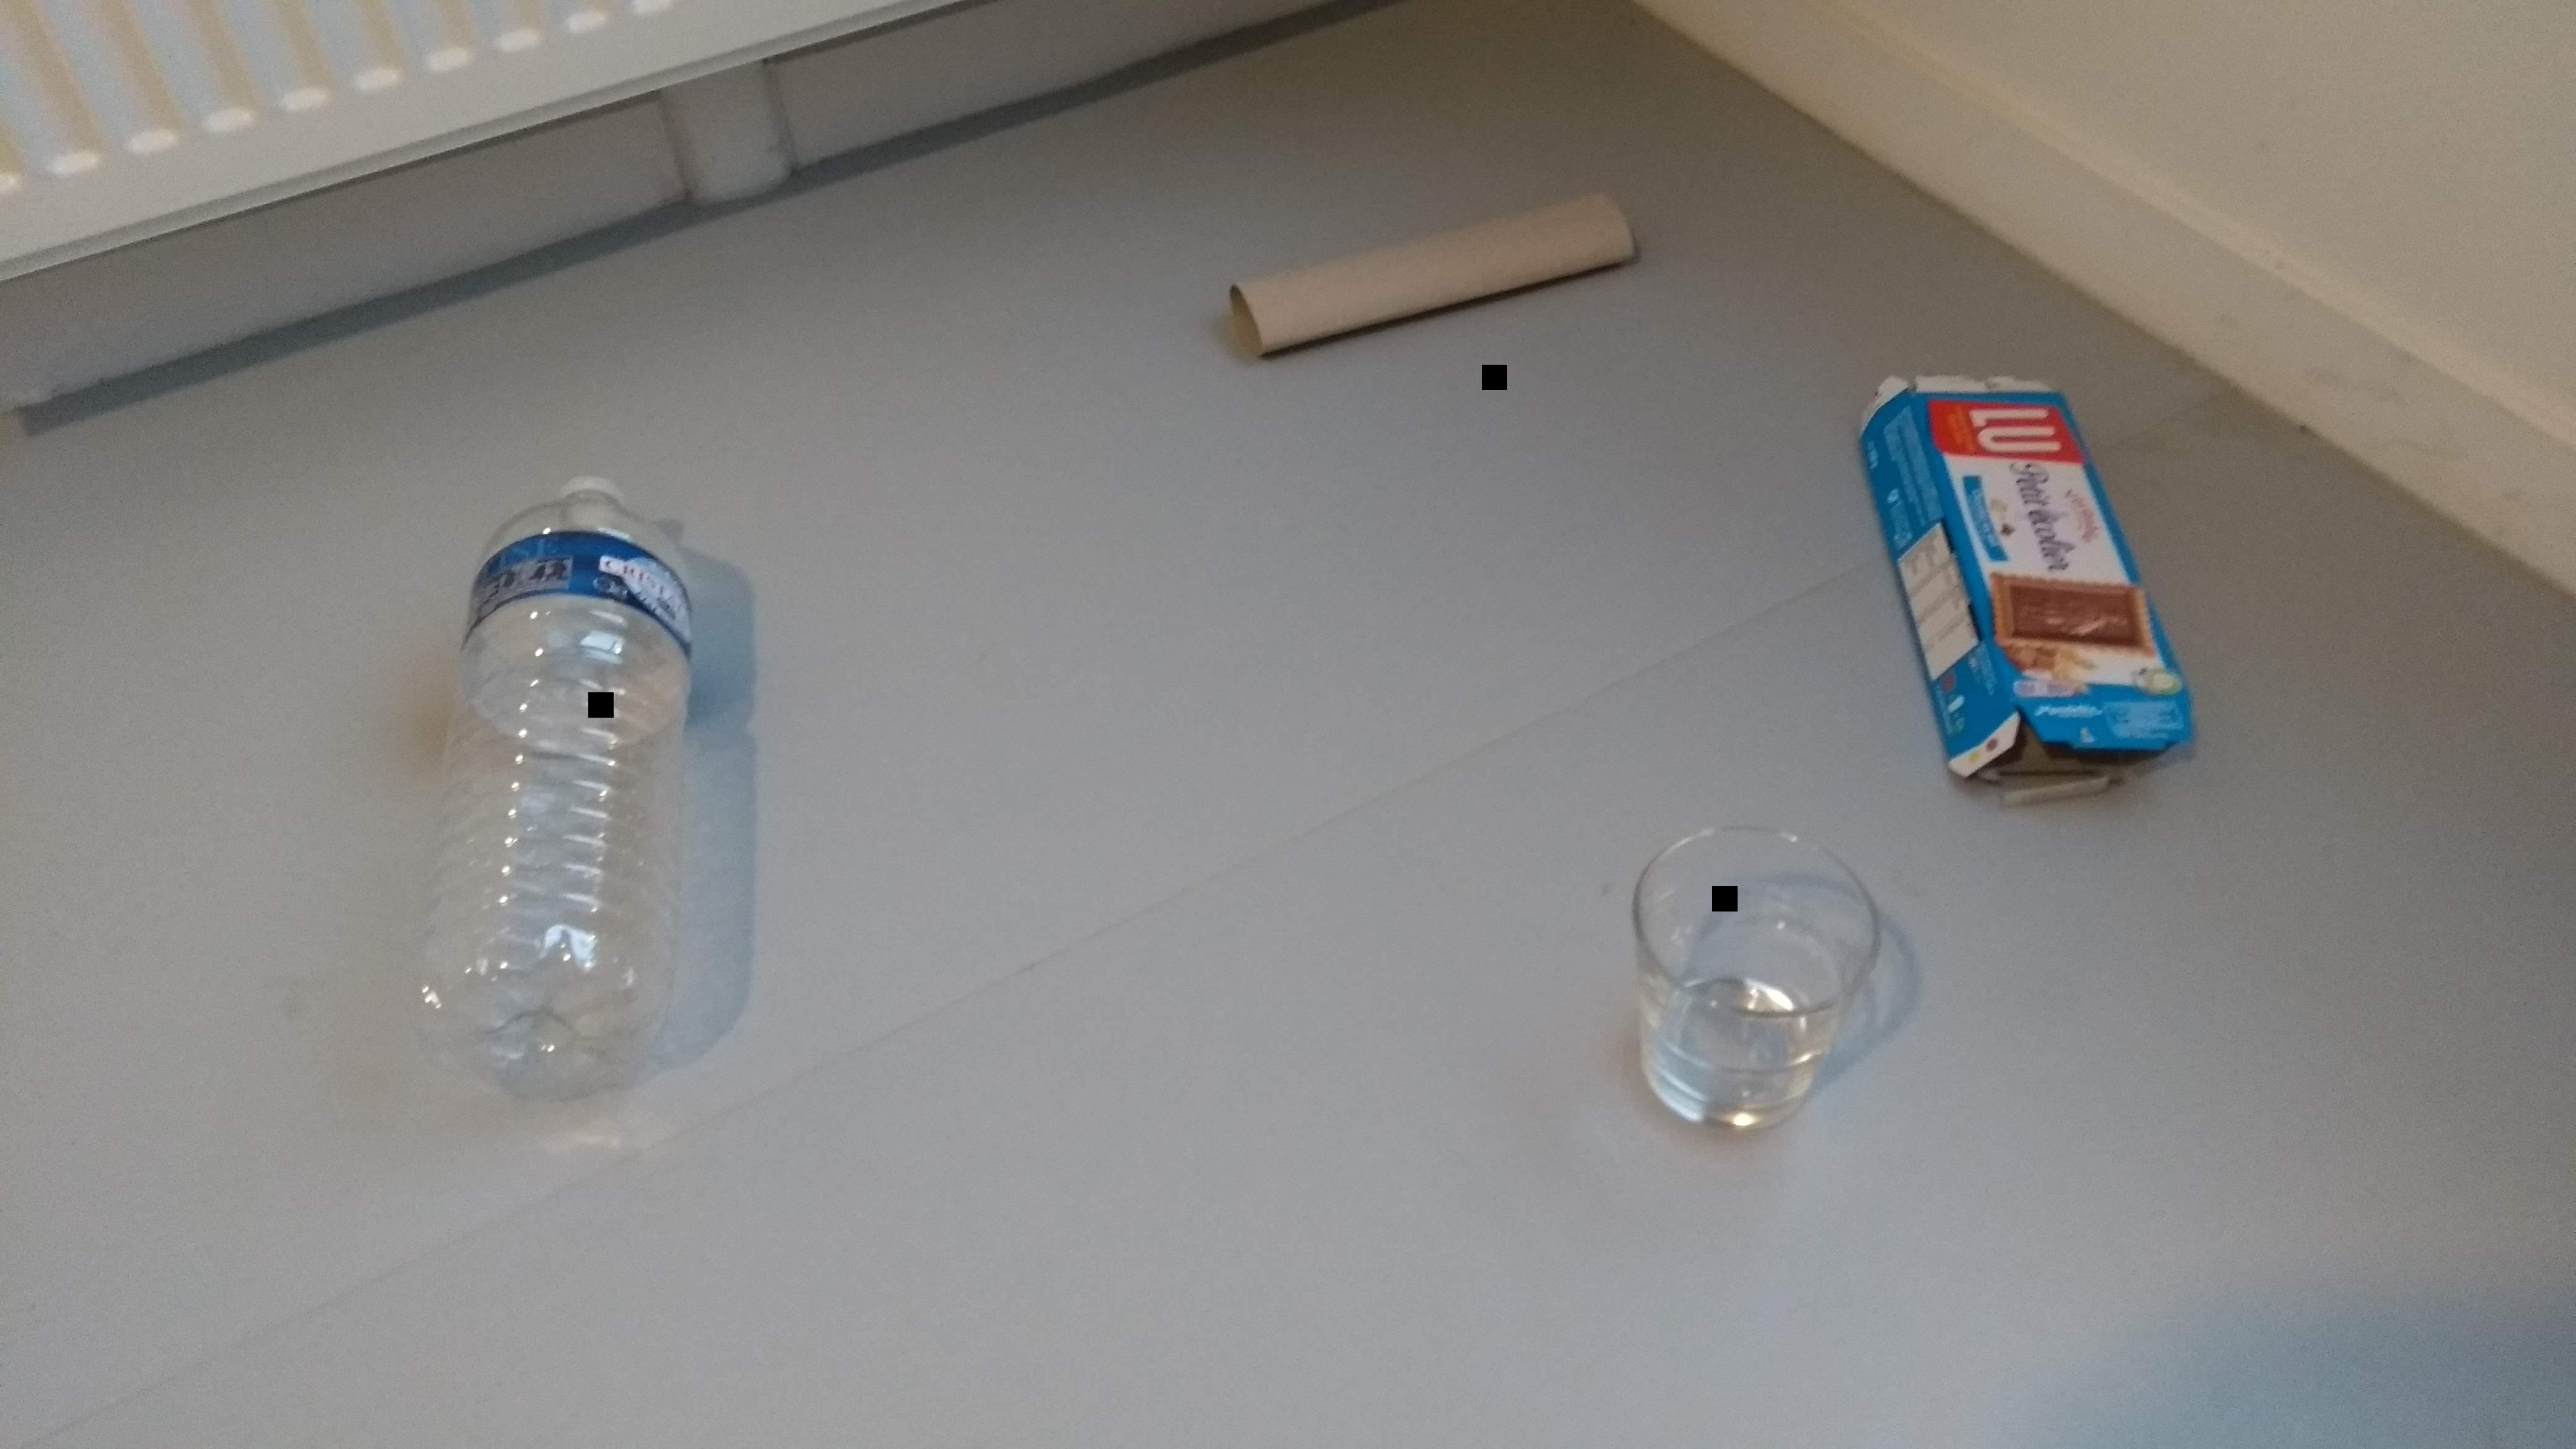
\includegraphics[width=7cm]{result.jpg}
	\caption{Test du réseau}
	\label{result}
\end{figure}



\section{Ce que nous allons faire maintenant}

\paragraph*{}

Dans les semaines qui vont suivre, nous allons nous nous concentrer sur trois points :
\begin{itemize}
  \item Tout d’abord, nous allons chercher à exploiter la première sortie du réseau Inception, afin d’améliorer et d’accélérer la détection sur une image avec plusieurs déchets non centrés.
  \item Nous allons ensuite chercher de rajouter une étape au réentraînement du réseau, ou nous défreezerons toutes les couches.
  \item Enfin, nous chercherons à agrandir notre BDD, soit en en trouvant une autre, soit en développant un scrapper pour google images.
\end{itemize}


\end{document}